\chapter{Interfaz y resultados finales}
\label{cap:Interfaz y resultados finales}

Con esto la interfaz se ve de la siguiente forma: 

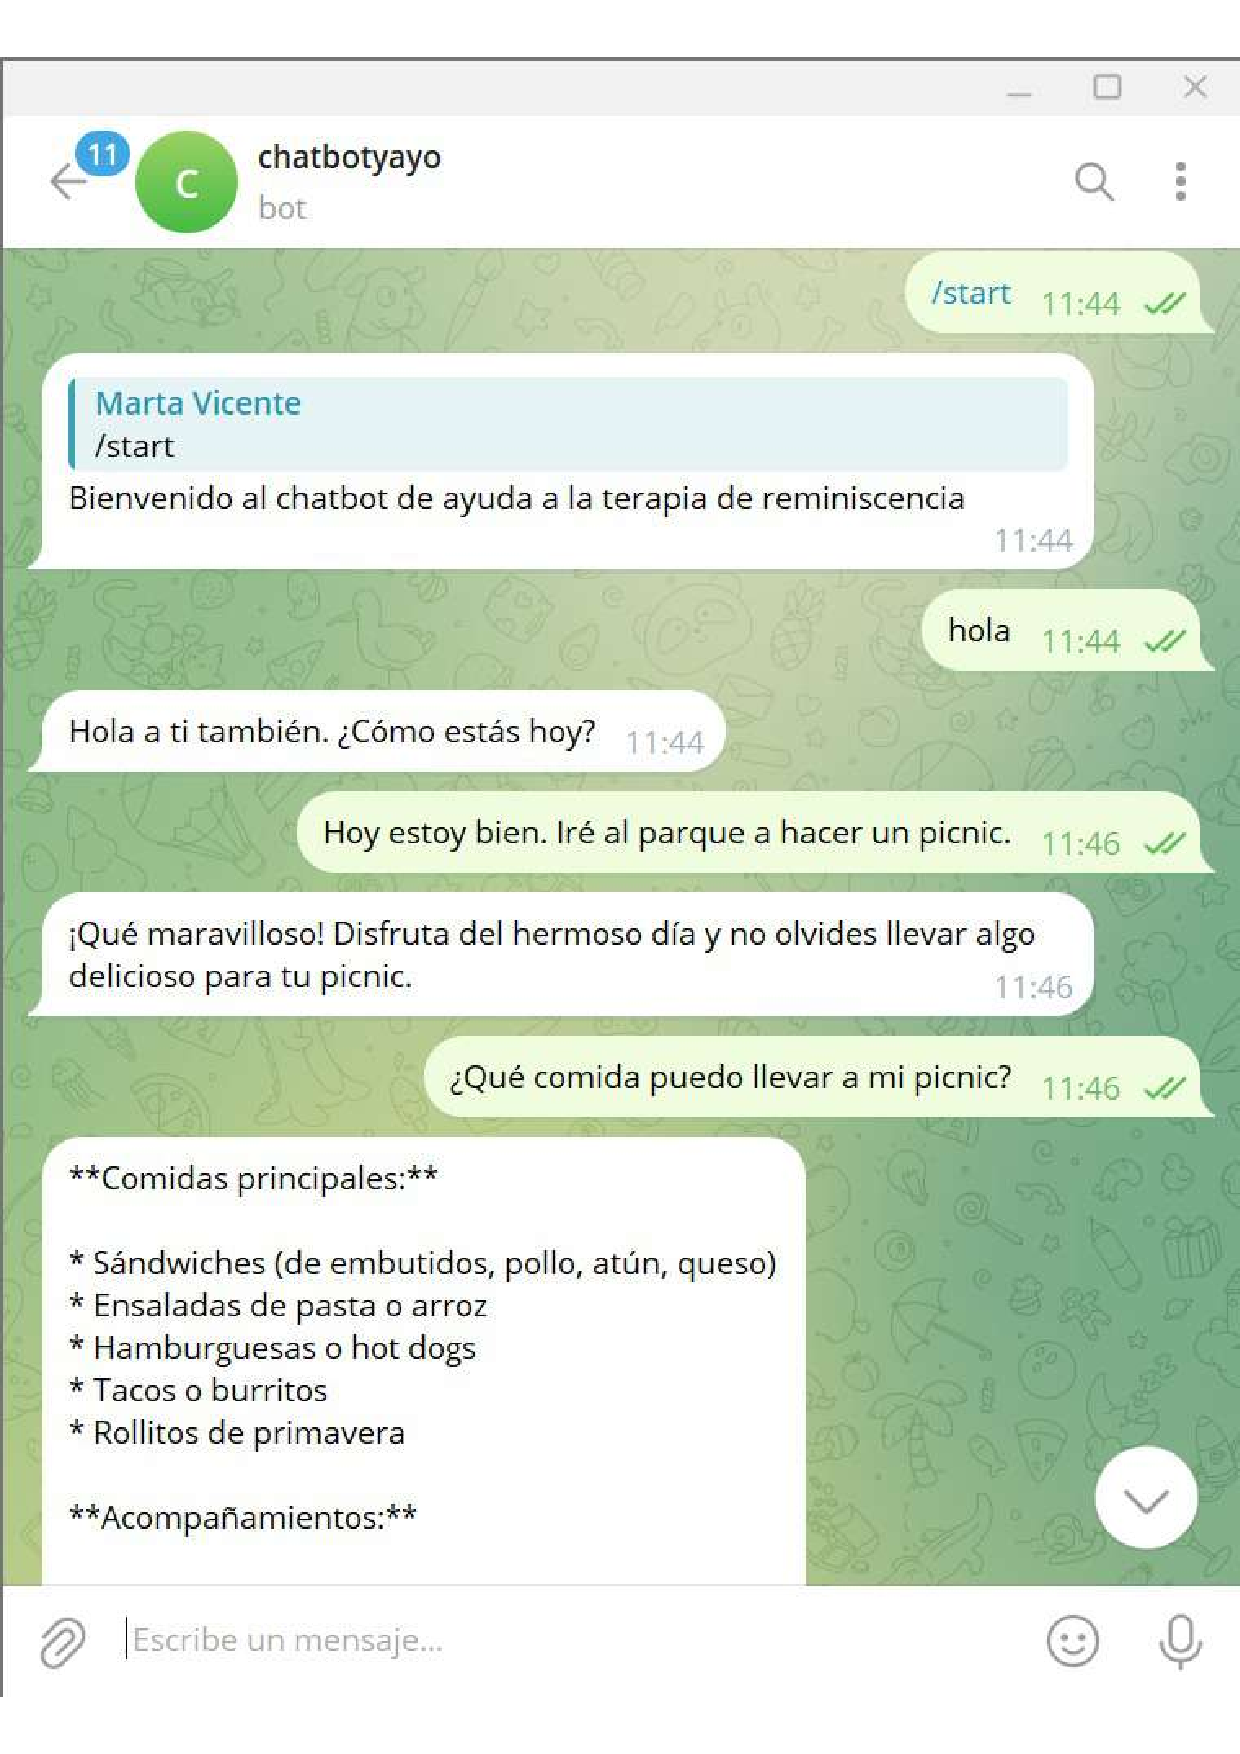
\includegraphics[width=0.5\textwidth]{Imagenes/telegram1}

%PRIMERA VERSIÓN EN BARD
%PRIMERA VERSIÓN EN GEMMA
%PRIMERA VERSIÓN GEMINI - GOOGLE COLLABORATE
%REFACTORIZACIÓN PARA HACER VERSIÓN LOCAL
%TELEGRAM
%GENERAR LAS ETAPAS 
%IMAGENES
%WHISPER
%GRÁFOS
%GENERACIÓN DE HISTORIAS DE VIDA
Para configurarlo, en primer lugar hay que ejecutar el programa mibot.py estando en telegram en la conversaa conversación de telegram el comando /start para comenzar la conversación y ya. 

Sin embago, y pese a las grandes funcionalidades de todas estas alternativas nos hemos decantado por hacer una interfaz con telegram desarrollando nuestro propio chatbot usando rasa. 

Para desarrollar el chatbot de telegram me he decantado por usar la interfaz de telegram para la cuál se necesita la API de Rasa. Las principales ventajas que ofrece esta herramienta es la facilidad del manejo de la interfaz pues telegram es una herramienta muy conocida con la que los terapeutas pueden estar más familiarizados. Además, esto nos permite también usar la versión del chatbotyayo para móvil. 

Para crear está interfaz hay que: 
1. Instalar rasa
2. Instalar telegram 
2. Obtener una api de rasa
4. crear un nuevo chatbot desde telegram con @botFather
5. Enviar a tu chatbot el comando /start

Una vez seguidos todos estos pasos ya puedes comenzar a interactuar con la API de rasa. 


